\documentclass[unknownkeysallowed]{beamer}
\usepackage[french,english]{babel}
\usepackage{beamer_js}
\usepackage{shortcuts_js}
\addbibresource{biblio.bib}
\usepackage{csquotes}
\begin{document}

%%%%%%%%%%%%%%%%%%%%%%%%%%%%%%%%%%%%%%%%%%%%%%%%%%%%%%%%%%%%%%%%%%%%%%%%%%%%%%%
%%%%%%%%%%%%%%%%%%%%%%             Headers               %%%%%%%%%%%%%%%%%%%%%%
%%%%%%%%%%%%%%%%%%%%%%%%%%%%%%%%%%%%%%%%%%%%%%%%%%%%%%%%%%%%%%%%%%%%%%%%%%%%%%%



%%%%%%%%%%%%%%%%%%%%%%%%%%%%%%%%%%%%%%%%%%%%%%%%%%%%%%%%%%%%%%%%%%%%%%%%%%%%%%%
\begin{frame}
\bigskip
\bigskip
\begin{center}{
\LARGE\color{marron}
\textbf{HMMA 307 : Modèles linéaires avancés}
\textbf{ }\\
\vspace{0.5cm}
}

\color{marron}
\textbf{Linear mixed effects models}
\end{center}

\vspace{0.5cm}

\begin{center}
\textbf{Cassandre Lepercque} \\
\vspace{0.1cm}
\url{https://github.com/cassandrelepercque/HMMA_307-Project}\\
\vspace{0.5cm}
Université de Montpellier \\
\end{center}

\centering

\includegraphics[width=0.13\textwidth]{Logo.pdf}

\end{frame}
%%%%%%%%%%%%%%%%%%%%%%%%%%%%%%%%%%%%%%%%%%%%%%%%%%%%%%%%%%%%%%%%%%%%%%%%%%%%%%%



%%%%%%%%%%%%%%%%%%%%%%%%%%%%%%%%%%%%%%%%%%%%%%%%%%%%%%%%%%%%%%%%%%%%%%%%%%%%%%%
%%%%%%%%%%%%%%%%%%%%%%%%       PLAN      %%%%%%%%%%%%%%%%%%%%%%%%%%%%%%%%%%%%%%
%%%%%%%%%%%%%%%%%%%%%%%%%%%%%%%%%%%%%%%%%%%%%%%%%%%%%%%%%%%%%%%%%%%%%%%%%%%%%%%

%%%%%%%%%%%%%%%%%%%%%%%%%%%%%%%%%%%%%%%%%%%%%%%%%%%%%%%%%%%%%%%%%%%%%%%%%%%%%%%
\begin{frame}{Table of Contents}
\tableofcontents[hideallsubsections]
\end{frame}
%%%%%%%%%%%%%%%%%%%%%%%%%%%%%%%%%%%%%%%%%%%%%%%%%%%%%%%%%%%%%%%%%%%%%%%%%%%%%%%


%%%%%%%%%%%%%%%%%%%%%%%%%%%%%%%%%%%%%%%%%%%%%%%%%%%%%%%%%%%%%%%%%%%%%%%%%%%%%%%
\AtBeginSection[]
{
\begin{frame}<beamer>{Table of Contents}
\tableofcontents[currentsubsection,
    hideothersubsections,
    sectionstyle=show/shaded,
]
\end{frame}
}
%%%%%%%%%%%%%%%%%%%%%%%%%%%%%%%%%%%%%%%%%%%%%%%%%%%%%%%%%%%%%%%%%%%%%%%%%%%%%%%

%%%%%%%%%%%%%%%%%%%%%%%%%%%%%%%%%%%%%%%%%%%%%%%%%%%%%%%%%%%%%%%%%%%%%%%%%%%%%%%
%%%%%%%%%%%%%%%%%%%%%%%%%%%%%%%%%%%%%%%%%%%%%%%%%%%%%%%%%%%%%%%%%%%%%%%%%%%%%%%
\section{Introduction}
\label{sec:Introduction}
%%%%%%%%%%%%%%%%%%%%%%%%%%%%%%%%%%%%%%%%%%%%%%%%%%%%%%%%%%%%%%%%%%%%%%%%%%%%%%
%%%%%%%%%%%%%%%%%%%%%%%%%%%%%%%%%%%%%%%%%%%%%%%%%%%%%%%%%%%%%%%%%%%%%%%%%%%%%%%

%%%%%%%%%%%%%%%%%%%%%%%%%%%%%%%%%%%%%%%%%%%%%%%%%%%%%%%%%%%%%%%%%%%%%%%%%%%%%%%
\subsection{Definition of Linear mixed effects models}
\label{sub:Definition of Linear mixed effects models}
%%%%%%%%%%%%%%%%%%%%%%%%%%%%%%%%%%%%%%%%%%%%%%%%%%%%%%%%%%%%%%%%%%%%%%%%%%%%%%%

%%%%%%%%%%%%%%%%%%%%%%%%%%%%%%%%%%%%%%%%%%%%%%%%%%%%%%%%%%%%%%%%%%%%%%%%%%%%%%%
\begin{frame}{Linear mixed effect models}

\mytheorem{Matrix model equation}
{\[y = X \beta + Z u + \epsilon\]}

\medskip

where,
\begin{itemize}
    \item $y$ is  a known vector of observations, with mean $\bbE[y]=X \beta$,
    \item $\beta$ is an unknown vector of fixed effects,
    \item $u$ is an unknown vector of random effects, with mean $\bbE[u] = 0$,
    \item $\epsilon$ is an unknown vector of random errors, with mean $\bbE[\epsilon]=0$,
    \item $X$ and $Z$ are known design matrices relating the observations $y$ to $\beta$ and $u$,  respectively.
\end{itemize}



\end{frame}
%%%%%%%%%%%%%%%%%%%%%%%%%%%%%%%%%%%%%%%%%%%%%%%%%%%%%%%%%%%%%%%%%%%%%%%%%%%%%%%

%%%%%%%%%%%%%%%%%%%%%%%%%%%%%%%%%%%%%%%%%%%%%%%%%%%%%%%%%%%%%%%%%%%%%%%%%%%%%%%
\subsection{Presentation of the dataset}
\label{sub:Presentation of the dataset}
%%%%%%%%%%%%%%%%%%%%%%%%%%%%%%%%%%%%%%%%%%%%%%%%%%%%%%%%%%%%%%%%%%%%%%%%%%%%%%%

%%%%%%%%%%%%%%%%%%%%%%%%%%%%%%%%%%%%%%%%%%%%%%%%%%%%%%%%%%%%%%%%%%%%%%%%%%%%%%%
\begin{frame}{Presentation of the dataset}
\vspace{0.5cm}
\textbf{Does the trophic position of fish increase with their size ?}
\begin{figure}
    \centering
    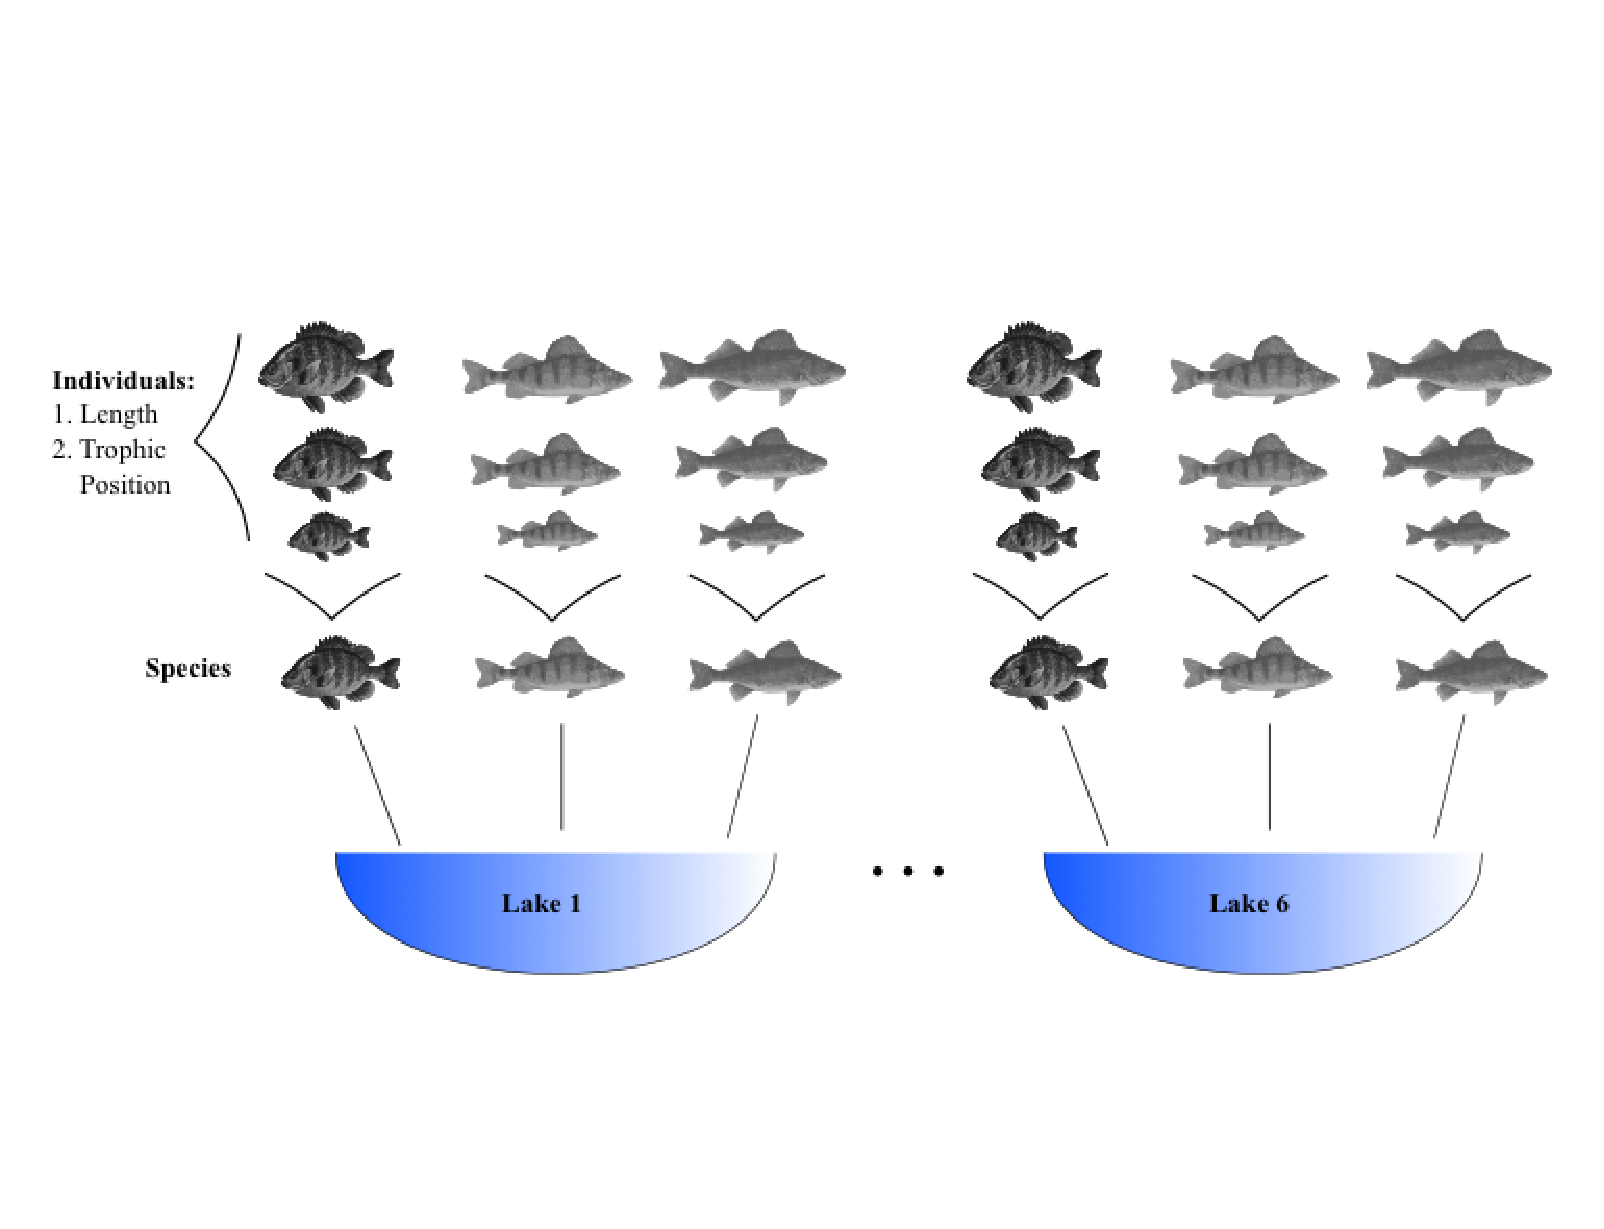
\includegraphics[scale=0.3]{image/fish_repartition.pdf}
    \caption{Dataset : Fish trophic position}
    \label{fig:my_label}
\end{figure}
\end{frame}

%%%%%%%%%%%%%%%%%%%%%%%%%%%%%%%%%%%%%%%%%%%%%%%%%%%%%%%%%%%%%%%%%%%%%%%%%%%%%%%
%%%%%%%%%%%%%%%%%%%%%%%%%%%%%%%%%%%%%%%%%%%%%%%%%%%%%%%%%%%%%%%%%%%%%%%%%%%%%%%
\section{Data analysis}
\label{sec:data analysis}
%%%%%%%%%%%%%%%%%%%%%%%%%%%%%%%%%%%%%%%%%%%%%%%%%%%%%%%%%%%%%%%%%%%%%%%%%%%%%%%
%%%%%%%%%%%%%%%%%%%%%%%%%%%%%%%%%%%%%%%%%%%%%%%%%%%%%%%%%%%%%%%%%%%%%%%%%%%%%%%

%%%%%%%%%%%%%%%%%%%%%%%%%%%%%%%%%%%%%%%%%%%%%%%%%%%%%%%%%%%%%%%%%%%%%%%%%%%%%%%
\subsection{Presentation model}
\label{sub:presentation model}
%%%%%%%%%%%%%%%%%%%%%%%%%%%%%%%%%%%%%%%%%%%%%%%%%%%%%%%%%%%%%%%%%%%%%%%%%%%%%%%

%%%%%%%%%%%%%%%%%%%%%%%%%%%%%%%%%%%%%%%%%%%%%%%%%%%%%%%%%%%%%%%%%%%%%%%%%%%%%%%
\begin{frame}{Model}
\mytheorem{The a priori model}
{\[TP_{ijk} \sim Length_i + Lake_j + Species_k + \epsilon\]}
\medskip
\begin{itemize}
    \item $TP_{ijk}$ is the trophic position of individual $i$ from lake $j$ of species $k$,
    \item $\epsilon$ are the residuals of the model.
\end{itemize}


\end{frame}
%%%%%%%%%%%%%%%%%%%%%%%%%%%%%%%%%%%%%%%%%%%%%%%%%%%%%%%%%%%%%%%%%%%%%%%%%%%%%%%

%%%%%%%%%%%%%%%%%%%%%%%%%%%%%%%%%%%%%%%%%%%%%%%%%%%%%%%%%%%%%%%%%%%%%%%%%%%%%%%
\begin{frame}{Boxplot 1}

\begin{figure}
    \centering
    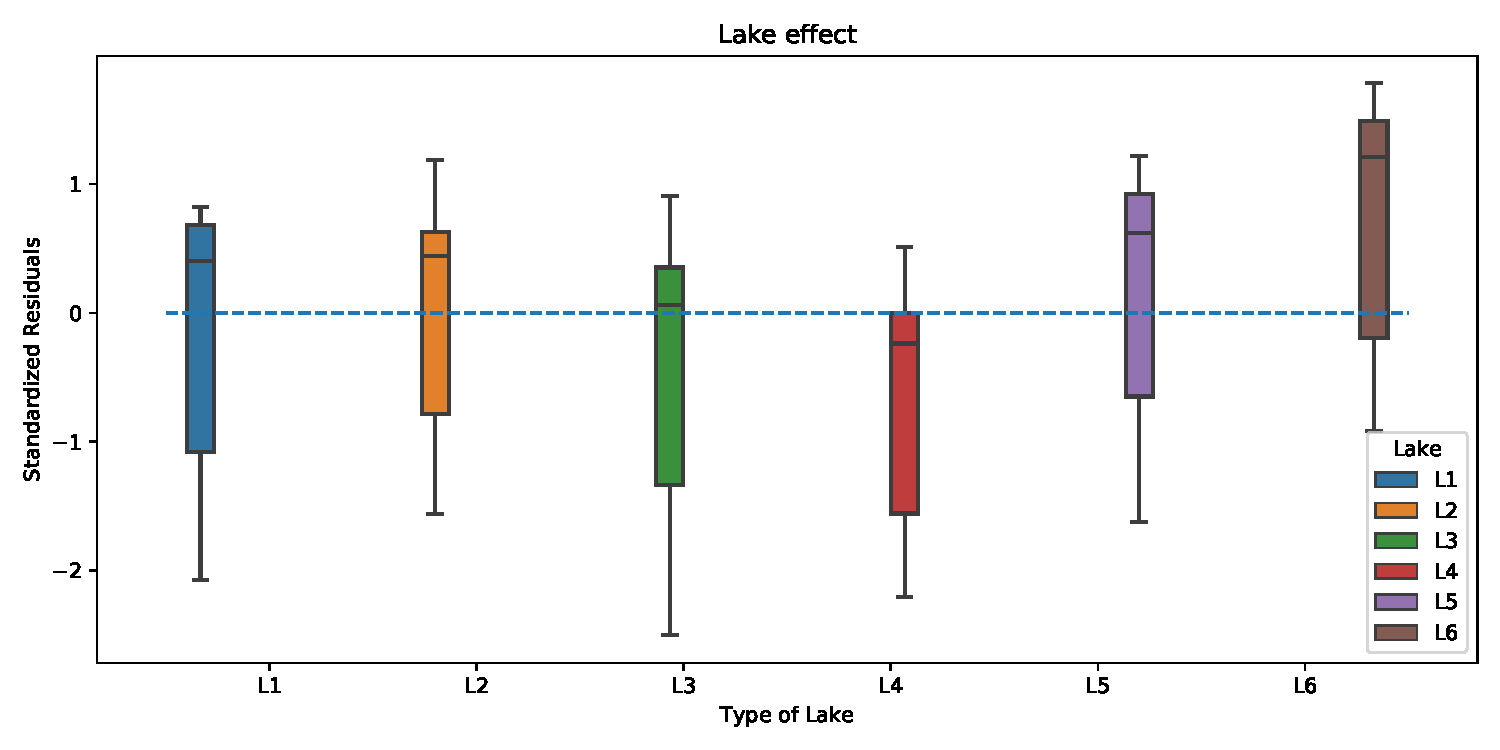
\includegraphics[scale=0.4]{image/boxplot_lake_effect.pdf}
    \caption{Boxplot of the lake effect}
    \label{fig:my_label}
\end{figure}


\end{frame}
%%%%%%%%%%%%%%%%%%%%%%%%%%%%%%%%%%%%%%%%%%%%%%%%%%%%%%%%%%%%%%%%%%%%%%%%%%%%%%%

%%%%%%%%%%%%%%%%%%%%%%%%%%%%%%%%%%%%%%%%%%%%%%%%%%%%%%%%%%%%%%%%%%%%%%%%%%%%%%%
\begin{frame}{Boxplot 2}

\begin{figure}
    \centering
    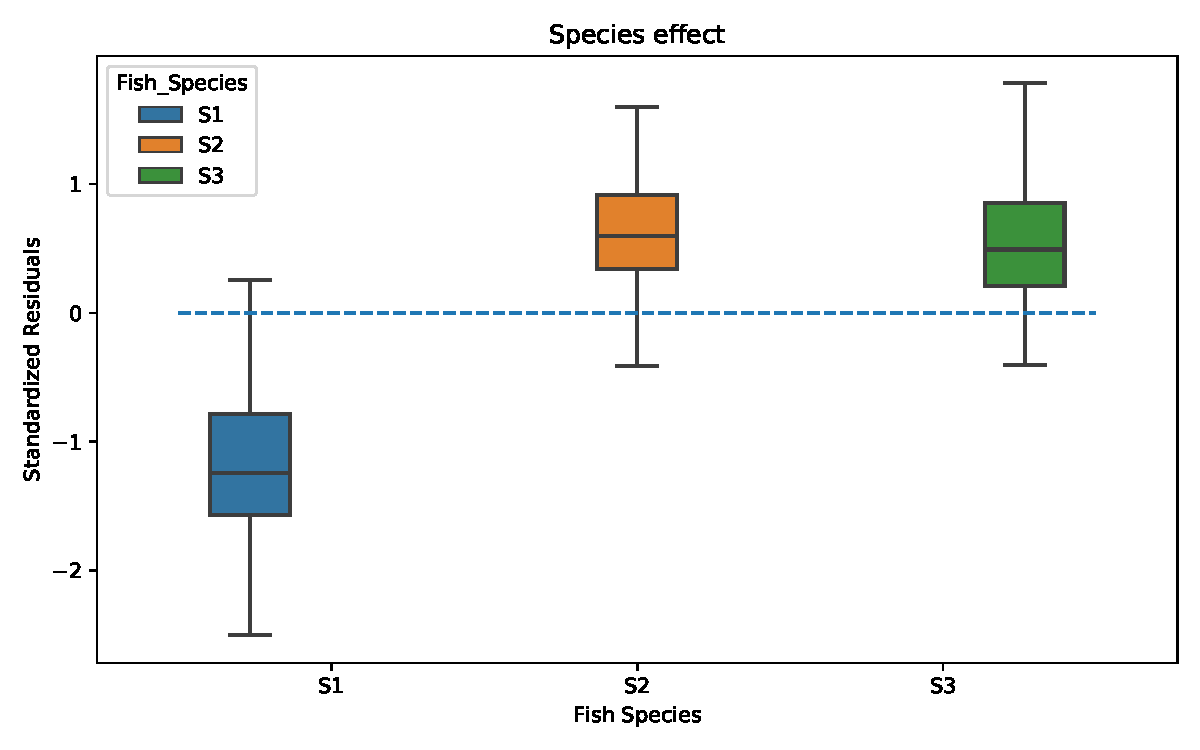
\includegraphics[scale=0.5]{image/boxplot_species_effect.pdf}
    \caption{Boxplot of the fish species effect}
    \label{fig:my_label}
\end{figure}


\end{frame}
%%%%%%%%%%%%%%%%%%%%%%%%%%%%%%%%%%%%%%%%%%%%%%%%%%%%%%%%%%%%%%%%%%%%%%%%%%%%%%%

%%%%%%%%%%%%%%%%%%%%%%%%%%%%%%%%%%%%%%%%%%%%%%%%%%%%%%%%%%%%%%%%%%%%%%%%%%%%%%%
\subsection{Models comparison}
\label{sub:model comparison}
%%%%%%%%%%%%%%%%%%%%%%%%%%%%%%%%%%%%%%%%%%%%%%%%%%%%%%%%%%%%%%%%%%%%%%%%%%%%%%%

%%%%%%%%%%%%%%%%%%%%%%%%%%%%%%%%%%%%%%%%%%%%%%%%%%%%%%%%%%%%%%%%%%%%%%%%%%%%%%%
\begin{frame}{The potential models}

\begin{itemize}
    \item \textbf{Model 1:} Linear model without random effect,
    \item \textbf{Model 2:} Complete model with different intercepts, 
    \item \textbf{Model 3:} Complete model with differents intercepts and slopes,
    \item \textbf{Model 4:} No Lake effect, random intercept only,
    \item \textbf{Model 5:} No Species effect, random intercept only
    \item \textbf{Model 6:} No Lake effect, random intercept and slope,
    \item \textbf{Model 7:} No Species effect, random intercept and slope,
    \item \textbf{Model 8:} Complete model with intercepts and slopes varying by lake, 
    \item \textbf{Model 9:} Complete model with intercepts and slopes varying by species.
\end{itemize}

\end{frame}
%%%%%%%%%%%%%%%%%%%%%%%%%%%%%%%%%%%%%%%%%%%%%%%%%%%%%%%%%%%%%%%%%%%%%%%%%%%%%%%

%%%%%%%%%%%%%%%%%%%%%%%%%%%%%%%%%%%%%%%%%%%%%%%%%%%%%%%%%%%%%%%%%%%%%%%%%%%%%%%
\begin{frame}{AIC Comparison}
\mytheorem{Akaike information criterion}
{\[AIC = deviance + 2\times (p+1)\]}
\medskip

Where, 
\begin{itemize}
    \item $deviance = - 2 \times (loglikelihood)$,
    \item $p$ = number of parameters.
\end{itemize}

\end{frame}
%%%%%%%%%%%%%%%%%%%%%%%%%%%%%%%%%%%%%%%%%%%%%%%%%%%%%%%%%%%%%%%%%%%%%%%%%%%%%%%

%%%%%%%%%%%%%%%%%%%%%%%%%%%%%%%%%%%%%%%%%%%%%%%%%%%%%%%%%%%%%%%%%%%%%%%%%%%%%%%
\begin{frame}{AIC Comparison}

\begin{table}[h!]
   \centering
    \begin{tabular}{ |p{1.5cm}||p{1.5cm}|p{1.5cm}|p{1cm}|p{1.5cm}|p{1.5cm}|}
    \hline
    \textbf{Models} & M1 & M2 & M3 & M4 & M5 \\
    \hline
     \textbf{AIC} & 480.726 & 113.490 & 69.178 & 280.069 & 460.434 \\ 
     \hline
    \end{tabular}
    \label{Tableau AIC}
\end{table}

\begin{table}[h!]
   \centering
    \begin{tabular}{ |p{1.5cm}||p{1.5cm}|p{1.5cm}|p{1.5cm}|p{1cm}|}
    \hline
    \textbf{Models} & M6 & M7 & M8 & M9\\
    \hline
     \textbf{AIC} & 270.557 & 462.406 & 125.754 & 64.757\\ 
     \hline
    \end{tabular}
    \caption{AIC of each model.}
    \label{Tableau AIC}
\end{table}

\end{frame}
%%%%%%%%%%%%%%%%%%%%%%%%%%%%%%%%%%%%%%%%%%%%%%%%%%%%%%%%%%%%%%%%%%%%%%%%%%%%%%%

%%%%%%%%%%%%%%%%%%%%%%%%%%%%%%%%%%%%%%%%%%%%%%%%%%%%%%%%%%%%%%%%%%%%%%%%%%%%%%%
\subsection{Model validation}
\label{sub:model validation}
%%%%%%%%%%%%%%%%%%%%%%%%%%%%%%%%%%%%%%%%%%%%%%%%%%%%%%%%%%%%%%%%%%%%%%%%%%%%%%%

%%%%%%%%%%%%%%%%%%%%%%%%%%%%%%%%%%%%%%%%%%%%%%%%%%%%%%%%%%%%%%%%%%%%%%%%%%%%%%%
\begin{frame}{Model validation: Homogeneity}

\begin{figure}
    \centering
    
\includegraphics[scale=0.6]{image/Model_validation_homo.pdf}
    \caption{Homogeneity}
    \label{fig:my_label}
\end{figure}

\end{frame}
%%%%%%%%%%%%%%%%%%%%%%%%%%%%%%%%%%%%%%%%%%%%%%%%%%%%%%%%%%%%%%%%%%%%%%%%%%%%%%%

%%%%%%%%%%%%%%%%%%%%%%%%%%%%%%%%%%%%%%%%%%%%%%%%%%%%%%%%%%%%%%%%%%%%%%%%%%%%%%%
\begin{frame}{Model validation: Independence}

\begin{figure}
    \centering
    
\includegraphics[scale=0.6]{image/Model_validation_ind.pdf}
    \caption{Independence}
    \label{fig:my_label}
\end{figure}

\end{frame}
%%%%%%%%%%%%%%%%%%%%%%%%%%%%%%%%%%%%%%%%%%%%%%%%%%%%%%%%%%%%%%%%%%%%%%%%%%%%%%%

%%%%%%%%%%%%%%%%%%%%%%%%%%%%%%%%%%%%%%%%%%%%%%%%%%%%%%%%%%%%%%%%%%%%%%%%%%%%%%%
\begin{frame}{Model validation: Independence}

\begin{figure}
    \centering
    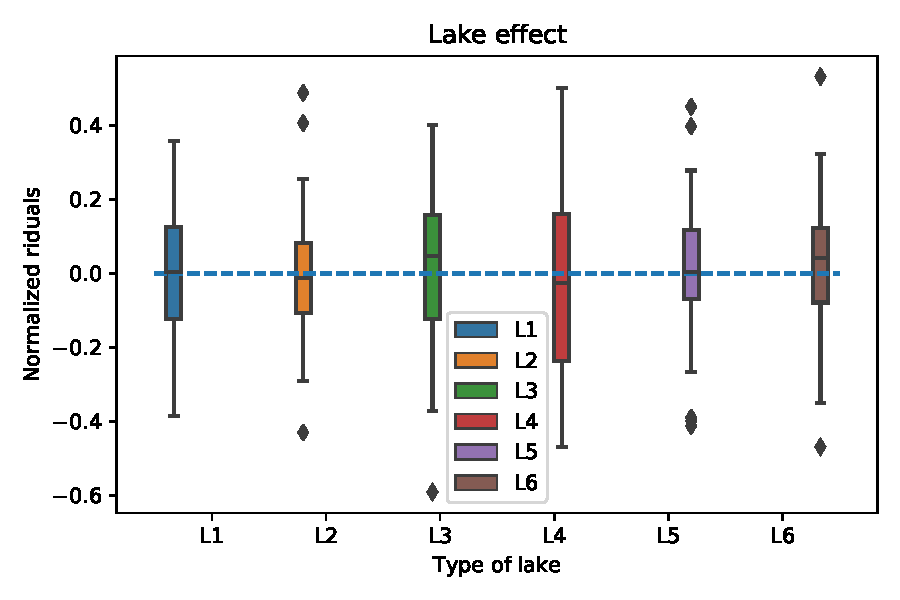
\includegraphics[scale=0.6]{image/boxplot_mod_vali_lake.pdf}
    \caption{Independence}
    \label{fig:my_label}
\end{figure}

\end{frame}
%%%%%%%%%%%%%%%%%%%%%%%%%%%%%%%%%%%%%%%%%%%%%%%%%%%%%%%%%%%%%%%%%%%%%%%%%%%%%%%

%%%%%%%%%%%%%%%%%%%%%%%%%%%%%%%%%%%%%%%%%%%%%%%%%%%%%%%%%%%%%%%%%%%%%%%%%%%%%%%
\begin{frame}{Model validation: Independence}

\begin{figure}
    \centering
    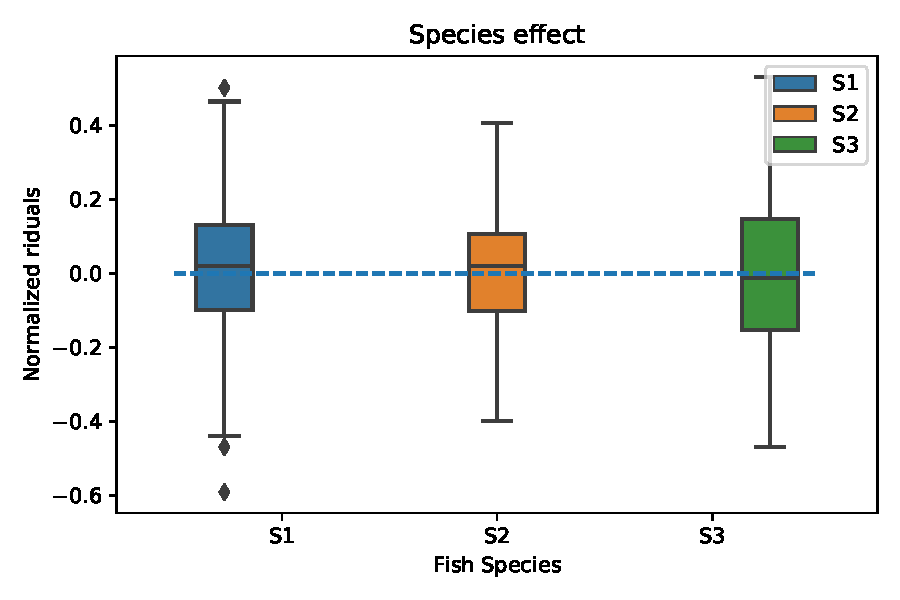
\includegraphics[scale=0.6]{image/boxplot_mod_vali_species.pdf}
    \caption{Independence}
    \label{fig:my_label}
\end{figure}

\end{frame}
%%%%%%%%%%%%%%%%%%%%%%%%%%%%%%%%%%%%%%%%%%%%%%%%%%%%%%%%%%%%%%%%%%%%%%%%%%%%%%%

%%%%%%%%%%%%%%%%%%%%%%%%%%%%%%%%%%%%%%%%%%%%%%%%%%%%%%%%%%%%%%%%%%%%%%%%%%%%%%%
\begin{frame}{Model validation: Normality}

\begin{figure}
    \centering
    
\includegraphics[scale=0.6]{image/hist_check_normality.pdf}
    \caption{Normality}
    \label{fig:my_label}
\end{figure}

\end{frame}
%%%%%%%%%%%%%%%%%%%%%%%%%%%%%%%%%%%%%%%%%%%%%%%%%%%%%%%%%%%%%%%%%%%%%%%%%%%%%%%

%%%%%%%%%%%%%%%%%%%%%%%%%%%%%%%%%%%%%%%%%%%%%%%%%%%%%%%%%%%%%%%%%%%%%%%%%%%%%%%
\section{Conclusion}
\label{sec:conclusion}
%%%%%%%%%%%%%%%%%%%%%%%%%%%%%%%%%%%%%%%%%%%%%%%%%%%%%%%%%%%%%%%%%%%%%%%%%%%%%%%
%%%%%%%%%%%%%%%%%%%%%%%%%%%%%%%%%%%%%%%%%%%%%%%%%%%%%%%%%%%%%%%%%%%%%%%%%%%%%%%


%%%%%%%%%%%%%%%%%%%%%%%%%%%%%%%%%%%%%%%%%%%%%%%%%%%%%%%%%%%%%%%%%%%%%%%%%%%%%%%%
\begin{frame}{Conclusion}
\begin{figure}
    \centering
    
\includegraphics[scale=0.6]{image/Model_visual_all_data.pdf}
    \caption{All data visualization}
    \label{fig:my_label}
\end{figure}
In our case, the trophic position increases with the size of the fish.\\
\vspace{1cm}
Mixed models are really good at accounting for variation in ecological data while not loosing too many degrees of freedom.\\
\end{frame}

%%%%%%%%%%%%%%%%%%%%%%%%%%%%%%%%%%%%%%%%%%%%%%%%%%%%%%%%%%%%%%%%%%%%%%%%%%%%%%%
%%%%%%%%%%%%%%%%%%%%%%%%%%%%%%%%%%%%%%%%%%%%%%%%%%%%%%%%%%%%%%%%%%%%%%%%%%%%%%%%
\begin{frame}{Conclusion}

Mixed models are really good at accounting for variation in ecological data while not loosing too many degrees of freedom.\\
\end{frame}

%%%%%%%%%%%%%%%%%%%%%%%%%%%%%%%%%%%%%%%%%%%%%%%%%%%%%%%%%%%%%%%%%%%%%%%%%%%%%%%

\end{document}